% Options for packages loaded elsewhere
\PassOptionsToPackage{unicode}{hyperref}
\PassOptionsToPackage{hyphens}{url}
%
\documentclass[
]{article}
\usepackage{lmodern}
\usepackage{amsmath}
\usepackage{ifxetex,ifluatex}
\ifnum 0\ifxetex 1\fi\ifluatex 1\fi=0 % if pdftex
  \usepackage[T1]{fontenc}
  \usepackage[utf8]{inputenc}
  \usepackage{textcomp} % provide euro and other symbols
  \usepackage{amssymb}
\else % if luatex or xetex
  \usepackage{unicode-math}
  \defaultfontfeatures{Scale=MatchLowercase}
  \defaultfontfeatures[\rmfamily]{Ligatures=TeX,Scale=1}
\fi
% Use upquote if available, for straight quotes in verbatim environments
\IfFileExists{upquote.sty}{\usepackage{upquote}}{}
\IfFileExists{microtype.sty}{% use microtype if available
  \usepackage[]{microtype}
  \UseMicrotypeSet[protrusion]{basicmath} % disable protrusion for tt fonts
}{}
\makeatletter
\@ifundefined{KOMAClassName}{% if non-KOMA class
  \IfFileExists{parskip.sty}{%
    \usepackage{parskip}
  }{% else
    \setlength{\parindent}{0pt}
    \setlength{\parskip}{6pt plus 2pt minus 1pt}}
}{% if KOMA class
  \KOMAoptions{parskip=half}}
\makeatother
\usepackage{xcolor}
\IfFileExists{xurl.sty}{\usepackage{xurl}}{} % add URL line breaks if available
\IfFileExists{bookmark.sty}{\usepackage{bookmark}}{\usepackage{hyperref}}
\hypersetup{
  hidelinks,
  pdfcreator={LaTeX via pandoc}}
\urlstyle{same} % disable monospaced font for URLs
\usepackage[margin=1in]{geometry}
\usepackage{longtable,booktabs}
\usepackage{calc} % for calculating minipage widths
% Correct order of tables after \paragraph or \subparagraph
\usepackage{etoolbox}
\makeatletter
\patchcmd\longtable{\par}{\if@noskipsec\mbox{}\fi\par}{}{}
\makeatother
% Allow footnotes in longtable head/foot
\IfFileExists{footnotehyper.sty}{\usepackage{footnotehyper}}{\usepackage{footnote}}
\makesavenoteenv{longtable}
\usepackage{graphicx}
\makeatletter
\def\maxwidth{\ifdim\Gin@nat@width>\linewidth\linewidth\else\Gin@nat@width\fi}
\def\maxheight{\ifdim\Gin@nat@height>\textheight\textheight\else\Gin@nat@height\fi}
\makeatother
% Scale images if necessary, so that they will not overflow the page
% margins by default, and it is still possible to overwrite the defaults
% using explicit options in \includegraphics[width, height, ...]{}
\setkeys{Gin}{width=\maxwidth,height=\maxheight,keepaspectratio}
% Set default figure placement to htbp
\makeatletter
\def\fps@figure{htbp}
\makeatother
\setlength{\emergencystretch}{3em} % prevent overfull lines
\providecommand{\tightlist}{%
  \setlength{\itemsep}{0pt}\setlength{\parskip}{0pt}}
\setcounter{secnumdepth}{-\maxdimen} % remove section numbering
\ifluatex
  \usepackage{selnolig}  % disable illegal ligatures
\fi

\author{}
\date{\vspace{-2.5em}}

\begin{document}

\textbf{Projeto LabEst: Consultoria em Análise Estatística para Alunos
de Pós-Graduação}

\textbf{Relatório Preliminar da Análise Estatística:}

Literacia Familiar no período pré e pandêmico de Covid-19: cenário
brasileiro e estratégias de intervenção

\textbf{Cliente}:

Natália Viana

Mestranda em Psicologia: Cognição e Comportamento - Faculdade de
Filosofia e Ciências Humanas da Universidade Federal de Minas Gerais

\textbf{Consultores}

Bianca Caravelli de Sá

Luiz Felipe Avelar

Thomás de Santiago Silva

Alunos da Disciplina ``Laboratório de Estatística I''

\textbf{Orientação: Prof.~Adrian Luna}

\textbf{15/07/2022}

\hypertarget{introduuxe7uxe3o-e-metodologia}{%
\subsection{\texorpdfstring{1) \textbf{Introdução e
metodologia}}{1) Introdução e metodologia}}\label{introduuxe7uxe3o-e-metodologia}}

O objetivo dessa tese de doutorado é investigar o impacto da pandemia de
COVID-19 nas práticas e recursos de literacia familiar no contexto
brasileiro, ou seja, investigar as práticas de leitura e letramento
feitas por pais e responsáveis com crianças pequenas feitas em casa
durante o período de quarentena e o impacto para o desenvolvimento da
alfabetização dessas crianças em um momento em que as escolas
encontravam-se fechadas.

Para a obtenção dos dados, foi aplicado o questionário ``Examinando a
influência das restrições da COVID-19 no ambiente de literacia
familiar'' que consiste em perguntas de interesse que descrevem o perfil
demográfico e socioeconômico dessas famílias, assim como os hábitos e
atividades de literacia desenvolvidas no ambiente familiar.

A partir desses dados obtidos no questionário, as análises do dados
encontram-se divididas em duas partes, a primeira consiste em uma
análise descritiva, através de gráficos de barra, histogramas, boxplots
e tabelas de frequência, das váriaveis de interesse principal que podem
impactar os hábitos de literacia durante a pandemia. Cada variável foi
analisada de maneira individual, sendo elas:

\begin{itemize}
\item
  Região de residência
\item
  Raça
\item
  Nível educacional do respondente
\item
  Nível Socioeconômico da família - renda familiar
\item
  Situação profissional do respondente antes e depois da covid
\item
  Quantidade de cuidadores
\item
  Quantidade de crianças
\item
  Tipo de quarentena
\item
  Nível de estresse com o isolamento
\end{itemize}

~~~~~~Já a segunda parte consiste em análises fatorial exploratórias a
partir de blocos de perguntas a fim de reduzir a quantidade de variávies
e obter indíces que explicam a variabilidade dos dados. As variáveis de
interesse para essa análise foram divididas nos seguintes blocos:

\begin{itemize}
\item
  Bloco 1 - Bloco Reading History Br (Histórico de alfabetização)
\item
  Bloco 2 - Home Literacy Resources Br (Recursos)
\item
  Bloco 3 - Enrichment Activities Br (Atividades de enriquecimento)
\end{itemize}

~\\

\hypertarget{anuxe1lise-exploratuxf3ria}{%
\subsection{\texorpdfstring{2) \textbf{Análise
Exploratória}}{2) Análise Exploratória}}\label{anuxe1lise-exploratuxf3ria}}

\hypertarget{regiuxe3o-de-residuxeancia}{%
\subsubsection{\texorpdfstring{\textbf{Região de
residência}}{Região de residência}}\label{regiuxe3o-de-residuxeancia}}

Pode-se observar que a grande maioria, 73,45\%, das pessoas que
respoderam ao questionário moram na região Sudeste do Brasil, enquanto
que apenas 2,55\% são residentes da região Centro-Oeste. Esta variável
possui 931 observações NAs.

\begin{figure}

{\centering \includegraphics{Relatório-Final-MCA-+-Descritiva-Final_files/figure-latex/unnamed-chunk-3-1} 

}

\caption{Figura 1 - Região de residência}\label{fig:unnamed-chunk-3}
\end{figure}

\hypertarget{rauxe7a}{%
\subsubsection{\texorpdfstring{\textbf{Raça}}{Raça}}\label{rauxe7a}}

Pode-se observar que 87,92\% das crianças são brancas ou pardas, sendo a
raça branca a mais frequente. Para esta variável houve 931 obervações
NAs.

\begin{figure}

{\centering 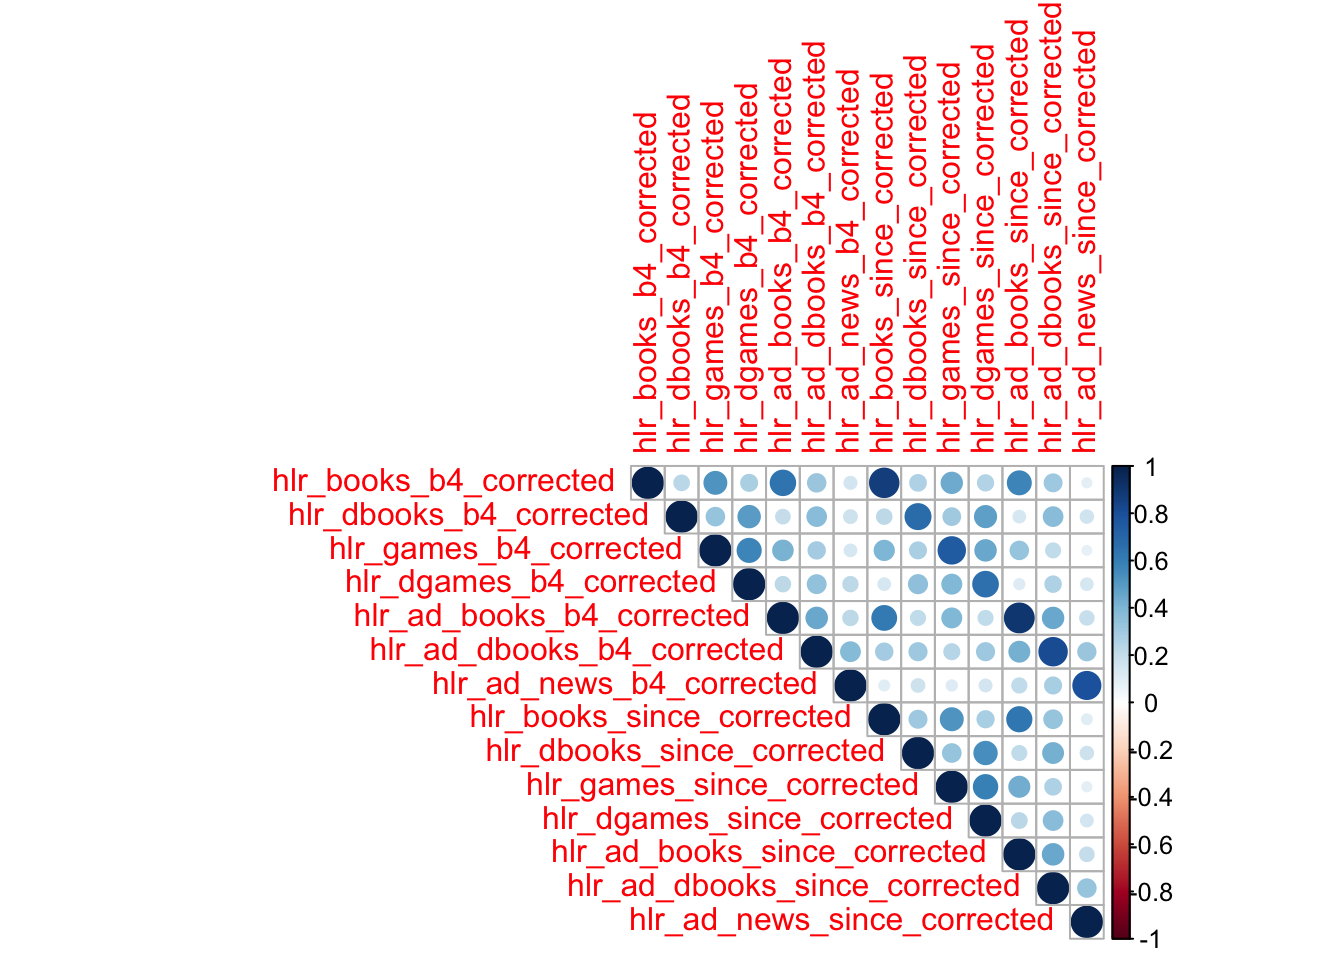
\includegraphics{Relatório-Final-MCA-+-Descritiva-Final_files/figure-latex/unnamed-chunk-4-1} 

}

\caption{Figura 2 - Raça}\label{fig:unnamed-chunk-4}
\end{figure}

\hypertarget{nuxedvel-educacional-do-respondente}{%
\subsubsection{\texorpdfstring{\textbf{Nível educacional do
respondente}}{Nível educacional do respondente}}\label{nuxedvel-educacional-do-respondente}}

Pode-se observar que a maioria dos respondentes do questionário possuem
um nível educacional alto, sendo que 51,55\% possuem pós-graduação,
enquanto que apenas 1,01\% dos respondentes possuiem Ensino Fundamental
completo ou incompleto.

Vale ressaltar que 931 pessoas não responderam a essa pergunta.

\begin{figure}

{\centering 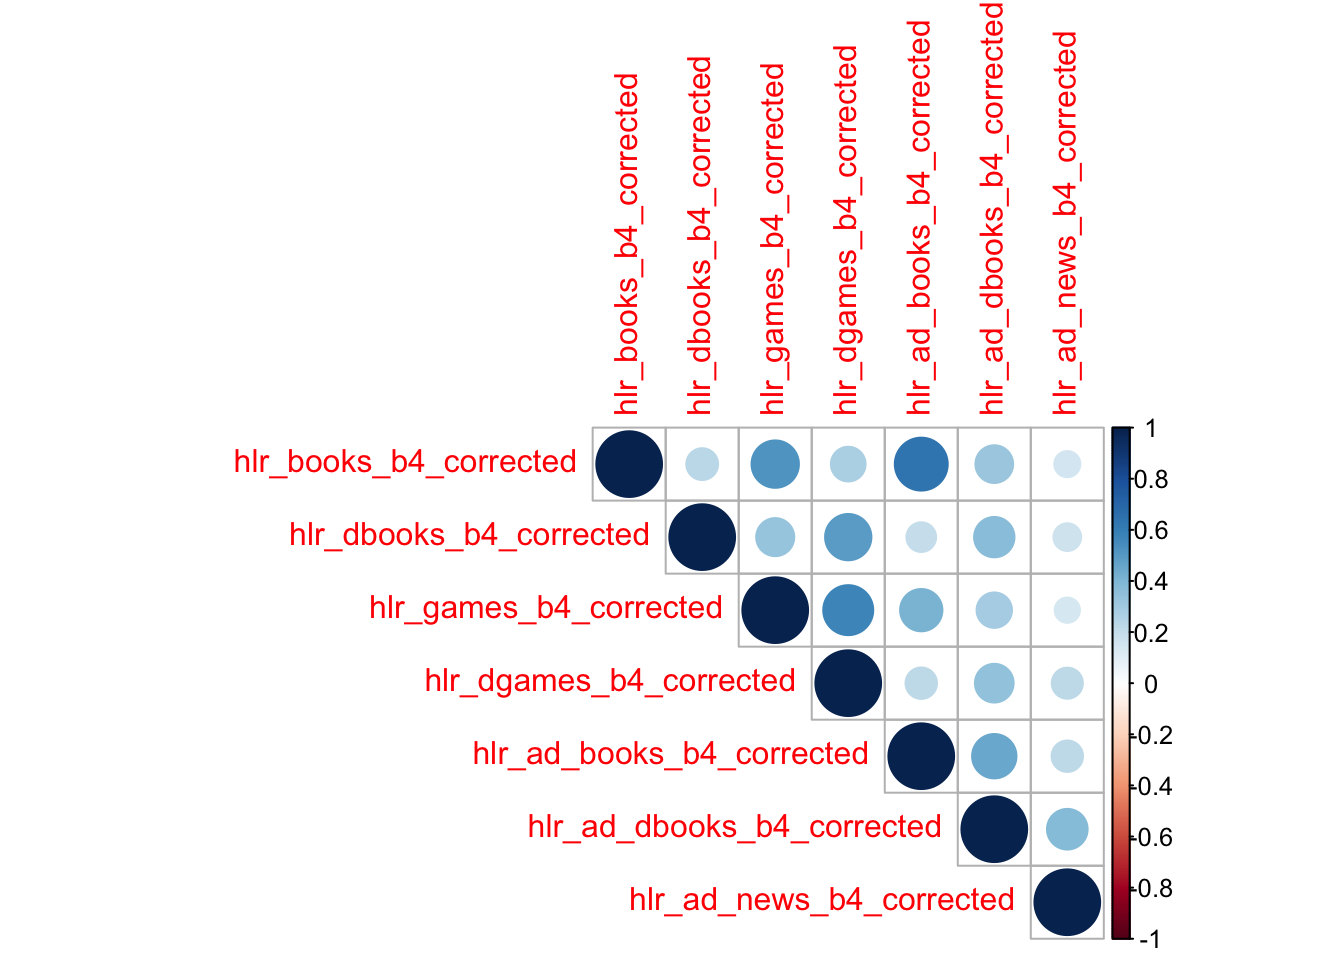
\includegraphics{Relatório-Final-MCA-+-Descritiva-Final_files/figure-latex/unnamed-chunk-6-1} 

}

\caption{Figura 3 - Nível educacional do respondente}\label{fig:unnamed-chunk-6}
\end{figure}

\hypertarget{nuxedvel-socioeconuxf4mico-da-famuxedlia---renda-familiar}{%
\subsubsection{\texorpdfstring{\textbf{Nível Socioeconômico da família -
Renda
familiar}}{Nível Socioeconômico da família - Renda familiar}}\label{nuxedvel-socioeconuxf4mico-da-famuxedlia---renda-familiar}}

Em relação a renda familiar, pode-se observar que possui uma
distribuição com consideráveis valores outliers, os gráficos abaixo
possuem duas versões, sendo a primeira os valores originais e a segunda
removendo os outliers. A renda mediana familiar é de R\$ 7000,00 e 978
pessoas não responderam a essa questão.

\begin{figure}

{\centering \includegraphics{Relatório-Final-MCA-+-Descritiva-Final_files/figure-latex/unnamed-chunk-8-1} 

}

\caption{Figura 4 - Renda familiar}\label{fig:unnamed-chunk-8}
\end{figure}

\begin{figure}

{\centering \includegraphics{Relatório-Final-MCA-+-Descritiva-Final_files/figure-latex/unnamed-chunk-9-1} 

}

\caption{Figura 5 - Renda familiar}\label{fig:unnamed-chunk-9}
\end{figure}

\hypertarget{situauxe7uxe3o-profissional-do-respondente-antes-e-depois-da-covid}{%
\subsubsection{\texorpdfstring{\textbf{Situação profissional do
respondente antes e depois da
covid}}{Situação profissional do respondente antes e depois da covid}}\label{situauxe7uxe3o-profissional-do-respondente-antes-e-depois-da-covid}}

Para as duas questões sobre situação profissional, há 12 opções de
resposta, sendo elas:

0 - Eu trabalhava em tempo integral fora de casa (mais do que 40 horas
por semana)

1 - Eu trabalhava em tempo integral em casa (mais do que 40 horas por
semana)

2 - Eu trabalhava em tempo integral, parcialmente em casa e parcialmente
fora de casa (mais do que 40 horas por semana)

3 - Eu trabalhava meio período fora de casa (menos que 40 horas por
semana)

4 - Eu trabalhava meio período em casa (menos que 40 horas por semana)

5 - Estudante

6 - Eu estava em licença de trabalho temporária (por exemplo suspenso do
trabalho, licença maternidade)

7 - Era dono(a) de casa ou cuidava das crianças em tempo integral

8 - Desempregado

9 - Aposentado

10 - Beneficiário do INSS

11 - Prefiro não responder

Pode-se observar que a grande maioria dos respondentes possuia um
emprego integral fora de casa anteriormente ao COVID-19, assim que a
pandemia se inicia há uma mudança na distribuição dos tipos de emprego e
o trabalho em casa passa a ser a categoria mais frequente.

\begin{verbatim}
## job_before : 
##         Frequency Percent Cum. percent
## 0             807   32.44        32.44
## 1             100    4.02        36.45
## 10              8    0.32        36.78
## 11             44    1.77        38.55
## 2             228    9.16        47.71
## 3             456   18.33        66.04
## 4              90    3.62        69.65
## 5             181    7.27        76.93
## 6              53    2.13        79.06
## 7             347   13.95        93.01
## 8             161    6.47        99.48
## 9              13    0.52       100.00
##   Total      2488  100.00       100.00
\end{verbatim}

\begin{verbatim}
## job_after : 
##         Frequency Percent Cum. percent
## 0             318   12.58        12.58
## 1             449   17.77        30.35
## 10              5    0.20        30.55
## 11             39    1.54        32.09
## 2             179    7.08        39.18
## 3             276   10.92        50.10
## 4             303   11.99        62.09
## 5             166    6.57        68.66
## 6              83    3.28        71.94
## 7             399   15.79        87.73
## 8             297   11.75        99.49
## 9              13    0.51       100.00
##   Total      2527  100.00       100.00
\end{verbatim}

\hypertarget{quantidade-de-cuidadores}{%
\subsubsection{\texorpdfstring{\textbf{Quantidade de
cuidadores}}{Quantidade de cuidadores}}\label{quantidade-de-cuidadores}}

Pode-se observar que das 2223 respostas ao questionário, 2085 respostas
foram de residências que possuem cuidadores.

\begin{verbatim}
## Quantidade_de_cuidadores : 
##         Frequency Percent Cum. percent
## 1             565   27.10        27.10
## 2             972   46.62        73.72
## 3             375   17.99        91.70
## 4             173    8.30       100.00
##   Total      2085  100.00       100.00
\end{verbatim}

\hypertarget{quantidade-de-crianuxe7as}{%
\subsubsection{\texorpdfstring{\textbf{Quantidade de
crianças}}{Quantidade de crianças}}\label{quantidade-de-crianuxe7as}}

Pode-se observar que a maioria das residências possuem duas ou menos
crianças, sendo que apenas 48 delas possuem quatro ou mais crianças.
Para esta variável há 47 observações NAs.

\begin{verbatim}
## Quantidade_de_criancas : 
##         Frequency Percent Cum. percent
## 1            1002   46.05        46.05
## 2             892   40.99        87.04
## 3             234   10.75        97.79
## 4              28    1.29        99.08
## 5              20    0.92       100.00
##   Total      2176  100.00       100.00
\end{verbatim}

\hypertarget{tipo-de-quarentena}{%
\subsubsection{\texorpdfstring{\textbf{Tipo de
quarentena}}{Tipo de quarentena}}\label{tipo-de-quarentena}}

Para o tipo de quarentena e restrições recomendadas à família, temos as
seguintes opções:

0 - Não há restrições agora

1 - Quarentena voluntária

2 - Pedido ou aviso depermanência em casa pelo governo local (caminhadas
ou passeios com distanciament osocial permitidos)

3 - Pedido de permanência em casa pelo governo local (só saia de casa
para fins essenciais)

4 - Outro

Pode-se observar que o tipo 3 foi o mais frequente, enquanto que o tipo
0 foi o menos frequente.

\begin{verbatim}
## restrictions : 
##         Frequency Percent Cum. percent
## Tipo 0        143    4.26         4.26
## Tipo 1        951   28.36        32.63
## Tipo 2        873   26.04        58.66
## Tipo 3       1343   40.05        98.72
## Tipo 4         43    1.28       100.00
##   Total      3353  100.00       100.00
\end{verbatim}

\hypertarget{nuxedvel-de-estresse-com-o-isolamento}{%
\subsubsection{\texorpdfstring{\textbf{Nível de estresse com o
isolamento}}{Nível de estresse com o isolamento}}\label{nuxedvel-de-estresse-com-o-isolamento}}

Para o nível de estresse com o isolamento, tem-se as seguintes
categorias:

0 - Não tem - Não tem sido estressante

1 - Pouco - Um pouco estressante

2 - Estressante - Estressante

3 - Muito - Muito estressante

4 - Extremamente - Extremamente estressante

Pode-se notar que apenas 175 das respostas consideram que o isolamento
não tem sido estressante, enquanto 712 o consideram pouco estressante.

\begin{verbatim}
## stress : 
##              Frequency Percent Cum. percent
## Estressante        483   22.98        22.98
## Extremamente       300   14.27        37.25
## Muito              432   20.55        57.80
## Não tem            175    8.33        66.13
## Pouco              712   33.87       100.00
##   Total           2102  100.00       100.00
\end{verbatim}

\hypertarget{anuxe1lise-fatorial---pca-e-mca}{%
\subsection{\texorpdfstring{3) \textbf{Análise Fatorial - PCA e
MCA}}{3) Análise Fatorial - PCA e MCA}}\label{anuxe1lise-fatorial---pca-e-mca}}

Ao trabalhar com um grande número de variáveis, a matriz de correlação
agrupa uma grande quantidade de coeficientes (190 coeficientes para K =
20 variáveis). É, portanto, essencial ter uma ferramenta capaz de
resumir as principais relações entre as variáveis de forma visual.

O objetivo do \textbf{PCA} é tirar conclusões das relações lineares
entre variáveis detectando as dimensões principais de variabilidade.
Como será analisado, estas conclusões serão complementadas pela
definição das variáveis sintéticas oferecidas pelo PCA. Portanto, será
mais fácil descrever os dados usando algumas variáveis sintéticas em vez
de todas as variáveis originais.

Assim como na análise de componentes principais (PCA), o objetivo é
resumir as relações entre as variáveis. Essas relações são estudadas em
pares ou todas juntas. Neste último caso, procuramos variáveis
sintéticas que resumem as informações contidas em um número de
variáveis. A informação transportada por uma variável pode ser estudada
em termosde suas categorias. Na \textbf{MCA}, focamos principalmente no
estudo das categorias, como categorias representam tanto variáveis
quanto um grupo de indivíduos (todos os indivíduos que selecionam esta
categoria).

\hypertarget{bloco-1---histuxf3rico-de-alfabetizauxe7uxe3o}{%
\subsubsection{\texorpdfstring{\textbf{Bloco 1 - Histórico de
alfabetização}}{Bloco 1 - Histórico de alfabetização}}\label{bloco-1---histuxf3rico-de-alfabetizauxe7uxe3o}}

\begin{longtable}[]{@{}ll@{}}
\toprule
Pré Covid & Com Covid\tabularnewline
\midrule
\endhead
rh\_read\_b4\_yng\_br & rh\_read\_since\_yng\_br\tabularnewline
rh\_read\_b4\_old\_br & rh\_read\_since\_old\_br\tabularnewline
rh\_read\_with\_b4\_old\_br & rh\_read\_w\_since\_old\_br\tabularnewline
rh\_readin\_b4\_old\_br & rh\_readin\_since\_old\_br\tabularnewline
rh\_read\_time\_b4\_br & rh\_read\_time\_since\_br\tabularnewline
\bottomrule
\end{longtable}

\begin{quote}
Correlação entre as variáveis do bloco:
\end{quote}

\begin{center}\includegraphics{Relatório-Final-MCA-+-Descritiva-Final_files/figure-latex/unnamed-chunk-21-1} \end{center}

\hypertarget{multiple-correspondence-analysis}{%
\subsubsection{\texorpdfstring{\textbf{Multiple Correspondence
Analysis}}{Multiple Correspondence Analysis}}\label{multiple-correspondence-analysis}}

O MCA geralmente é usado para analisar um conjunto de dados de uma
pesquisa. O objetivo é identificar:

1 - Um grupo de indivíduos com perfil semelhante em suas respostas às
perguntas

2 - As associações entre categorias de variáveis

Calcular e visualizar a análise de correspondência múltipla no software
R usando \emph{FactoMineR} (para a análise) e \emph{factoextra} (para
visualização de dados).

Revelar as variáveis mais importantes que mais contribuem para explicar
as variações no conjunto de dados explicando como prever os resultados
para indivíduos e variáveis suplementares. Filtrar os resultados do MCA
para manter apenas as variáveis que mais contribuíram.

\hypertarget{pruxe9-pandemia}{%
\paragraph{\texorpdfstring{\textbf{Pré
Pandemia}}{Pré Pandemia}}\label{pruxe9-pandemia}}

\begin{verbatim}
##  read_other read_u  read_with read_indep   read_time  
##  0: 58      0: 69   0:152     0:227      1      :376  
##  1:143      1:159   1:135     1:118      2      :138  
##  2:145      2:143   2:134     2: 78      8      : 60  
##  3: 56      3: 64   3: 54     3: 39      3      : 23  
##  4:151      4:112   4: 98     4: 93      7      : 10  
##  5: 50      5: 40   5: 23     5: 27      4      :  4  
##  6: 12      6: 28   6: 19     6: 33      (Other):  4
\end{verbatim}

\begin{center}\includegraphics{Relatório-Final-MCA-+-Descritiva-Final_files/figure-latex/unnamed-chunk-24-1} \end{center}

\begin{quote}
Construindo o MCA
\end{quote}

As variáveis podem ser representadas calculando as razões de correlação
entre as coordenadas dos indivíduos em um componente e cada uma das
categorias.

No gráfico biplot abaixo cada alternativa para cada resposta do
questionário é plotada em vermelho, enquanto que cada indivíduo (pessoa
que respondeu o questionário) é plotado em vermelho. Estas obervações
são plotadas em relação as duas dimensões mais explicativas, no caso as
dimensões 1 e 2 e indica o quão bem cada dimensão explica aquele
observação. Pode-se observar que há uma quantidade grande de indivíduos
no canto inferior esquerdo do gráfico que não são bem explicados por
pelas duas dimensões.

\begin{figure}

{\centering \includegraphics{Relatório-Final-MCA-+-Descritiva-Final_files/figure-latex/unnamed-chunk-26-1} 

}

\caption{Figura n - Representação do quanto as duas principais dimensões explicam cada dividuo e variavel}\label{fig:unnamed-chunk-26}
\end{figure}

\begin{quote}
Visualização e interpretação
\end{quote}

Estudar a inércia dos componentes principais permite-nos, por um lado,
ver se as variáveis estão estruturadas (presença de correlações entre
variáveis) e, além disso, determinar o número de componentes a serem
interpretados.

Os resultados em abaixo, produzidos em um gráfico de barras,
correspondem ao autovalor (ou seja, a inércia ou a variação explicada)
associada a cada um dos componentes; a porcentagem de inércia associada
a cada componente e a soma cumulativa dessas porcentagens.

\begin{quote}
Porcentagens de inércia explicadas por cada dimensão MCA
\end{quote}

\begin{figure}

{\centering \includegraphics{Relatório-Final-MCA-+-Descritiva-Final_files/figure-latex/unnamed-chunk-27-1} 

}

\caption{Figura n - Representação gráfica da porcentagem de variância explicada por cada dimensão}\label{fig:unnamed-chunk-27}
\end{figure}

\begin{quote}
Dentre das 15 principais categorias do gráfico anterior, o plot de
quanto elas contribuem para as duas maiores dimensões
\end{quote}

\begin{figure}

{\centering \includegraphics{Relatório-Final-MCA-+-Descritiva-Final_files/figure-latex/unnamed-chunk-28-1} 

}

\caption{Figura n - Representação do quanto cada altenativa do questionário contribui para as pricipais}\label{fig:unnamed-chunk-28-1}
\end{figure}
\begin{figure}

{\centering \includegraphics{Relatório-Final-MCA-+-Descritiva-Final_files/figure-latex/unnamed-chunk-28-2} 

}

\caption{Figura n - Representação do quanto cada altenativa do questionário contribui para as pricipais}\label{fig:unnamed-chunk-28-2}
\end{figure}

\begin{quote}
Correlação entre variáveis e dimensões principais
\end{quote}

\begin{center}\includegraphics{Relatório-Final-MCA-+-Descritiva-Final_files/figure-latex/unnamed-chunk-29-1} \end{center}

\hypertarget{puxf3s-pandemia}{%
\paragraph{\texorpdfstring{\textbf{Pós
Pandemia}}{Pós Pandemia}}\label{puxf3s-pandemia}}

\begin{verbatim}
##  read_other read_u  read_with read_indep   read_time  
##  0: 99      0:104   0:136     0:185      1      :346  
##  1:127      1:157   1:152     1:134      2      :114  
##  2:117      2:113   2:118     2: 77      8      : 85  
##  3: 74      3: 62   3: 64     3: 43      3      : 35  
##  4:143      4:109   4: 89     4: 91      4      : 13  
##  5: 34      5: 35   5: 31     5: 37      7      : 10  
##  6: 21      6: 35   6: 25     6: 48      (Other): 12
\end{verbatim}

\begin{center}\includegraphics{Relatório-Final-MCA-+-Descritiva-Final_files/figure-latex/unnamed-chunk-32-1} \end{center}

\begin{quote}
Construindo o MCA
\end{quote}

As variáveis podem ser representadas calculando as razões de correlação
entre as coordenadas dos indivíduos em um componente e cada uma das
categorias.

No gráfico biplot abaixo cada alternativa para cada resposta do
questionário é plotada em vermelho, enquanto que cada indivíduo (pessoa
que respondeu o questionário) é plotado em vermelho. Estas obervações
são plotadas em relação as duas dimensões mais explicativas, no caso as
dimensões 1 e 2 e indica o quão bem cada dimensão explica aquele
observação. Pode-se observar que há uma quantidade grande de indivíduos
no canto inferior esquerdo do gráfico que não são bem explicados por
pelas duas dimensões.

\begin{figure}

{\centering \includegraphics{Relatório-Final-MCA-+-Descritiva-Final_files/figure-latex/unnamed-chunk-34-1} 

}

\caption{Figura n - Representação do quanto as duas principais dimensões explicam cada dividuo e variavel}\label{fig:unnamed-chunk-34}
\end{figure}

\begin{quote}
Visualização e interpretação
\end{quote}

Estudar a inércia dos componentes principais permite-nos, por um lado,
ver se as variáveis estão estruturadas (presença de correlações entre
variáveis) e, além disso, determinar o número de componentes a serem
interpretados.

Os resultados em abaixo, produzidos em um gráfico de barras,
correspondem ao autovalor (ou seja, a inércia ou a variação explicada)
associada a cada um dos componentes; a porcentagem de inércia associada
a cada componente e a soma cumulativa dessas porcentagens.

\begin{quote}
Porcentagens de inércia explicadas por cada dimensão MCA
\end{quote}

\begin{figure}

{\centering \includegraphics{Relatório-Final-MCA-+-Descritiva-Final_files/figure-latex/unnamed-chunk-35-1} 

}

\caption{Figura n - Representação gráfica da porcentagem de variância explicada por cada dimensão}\label{fig:unnamed-chunk-35}
\end{figure}

\begin{quote}
Dentre das 15 principais categorias do gráfico anterior, o plot de
quanto elas contribuem para as duas maiores dimensões
\end{quote}

\begin{figure}

{\centering \includegraphics{Relatório-Final-MCA-+-Descritiva-Final_files/figure-latex/unnamed-chunk-36-1} 

}

\caption{Figura n - Representação do quanto cada altenativa do questionário contribui para as pricipais}\label{fig:unnamed-chunk-36-1}
\end{figure}
\begin{figure}

{\centering \includegraphics{Relatório-Final-MCA-+-Descritiva-Final_files/figure-latex/unnamed-chunk-36-2} 

}

\caption{Figura n - Representação do quanto cada altenativa do questionário contribui para as pricipais}\label{fig:unnamed-chunk-36-2}
\end{figure}

\begin{quote}
Correlação entre variáveis e dimensões principais
\end{quote}

\begin{center}\includegraphics{Relatório-Final-MCA-+-Descritiva-Final_files/figure-latex/unnamed-chunk-37-1} \end{center}

\hypertarget{bloco-2---recursos-de-alfabetizauxe7uxe3o-inicial}{%
\subsubsection{\texorpdfstring{\textbf{Bloco 2 - Recursos de
alfabetização
inicial}}{Bloco 2 - Recursos de alfabetização inicial}}\label{bloco-2---recursos-de-alfabetizauxe7uxe3o-inicial}}

\begin{longtable}[]{@{}ll@{}}
\toprule
Pré Covid & Com Covid\tabularnewline
\midrule
\endhead
hlr\_books\_b4\_corrected & hlr\_books\_since\_corrected\tabularnewline
hlr\_dbooks\_b4\_corrected &
hlr\_dbooks\_since\_corrected\tabularnewline
hlr\_games\_b4\_corrected & hlr\_games\_since\_corrected\tabularnewline
hlr\_dgames\_b4\_corrected &
hlr\_dgames\_since\_corrected\tabularnewline
hlr\_ad\_books\_b4\_corrected &
hlr\_ad\_books\_since\_corrected\tabularnewline
hlr\_ad\_dbooks\_b4\_corrected &
hlr\_ad\_dbooks\_since\_corrected\tabularnewline
hlr\_ad\_news\_b4\_corrected &
hlr\_ad\_news\_since\_corrected\tabularnewline
\bottomrule
\end{longtable}

\begin{quote}
Correlação entre as variáveis do bloco:
\end{quote}

Tanto para o bloco pré-pandemia como para o pós-pandemia, pode-se
observar que as variávies \textbf{books} \textbar{} \textbf{ad\_books} e
\textbf{games} \textbar{} \textbf{dgames} possuem a maior correlação,
indicando que, casas com uma maior quantidade de livros para crianças
tendem a ter também uma maior quantidade de livros para adultos. O mesmo
acontece entre jogos e jogos digitais.

Há correlações que aumentaram e outras que diminuiram no período
pandemico, no entanto, a maior diferença é de 0.08.

\begin{center}\includegraphics{Relatório-Final-MCA-+-Descritiva-Final_files/figure-latex/unnamed-chunk-39-1} \end{center}

\hypertarget{multiple-correspondence-analysis-1}{%
\subsubsection{\texorpdfstring{\textbf{Multiple Correspondence
Analysis}}{Multiple Correspondence Analysis}}\label{multiple-correspondence-analysis-1}}

O MCA geralmente é usado para analisar um conjunto de dados de uma
pesquisa. O objetivo é identificar:

1 - Um grupo de indivíduos com perfil semelhante em suas respostas às
perguntas

2 - As associações entre categorias de variáveis

Calcular e visualizar a análise de correspondência múltipla no software
R usando \emph{FactoMineR} (para a análise) e \emph{factoextra} (para
visualização de dados).

Revelar as variáveis mais importantes que mais contribuem para explicar
as variações no conjunto de dados explicando como prever os resultados
para indivíduos e variáveis suplementares. Filtrar os resultados do MCA
para manter apenas as variáveis que mais contribuíram.

\hypertarget{pruxe9-pandemia-1}{%
\paragraph{\texorpdfstring{\textbf{Pré
Pandemia}}{Pré Pandemia}}\label{pruxe9-pandemia-1}}

\begin{verbatim}
##     books_b4     dbooks_b4      games_b4     dgames_b4    ad_books_b4 
##  2      :240   0      :345   1      :404   1      :336   2      :181  
##  1      :160   1      :195   2      :117   0      :172   1      :147  
##  3      : 92   2      : 43   0      : 50   2      : 74   3      : 77  
##  7      : 46   3      : 10   3      : 18   3      : 19   7      : 67  
##  4      : 28   7      :  7   4      : 10   7      :  5   4      : 61  
##  0      : 21   4      :  6   5      :  7   4      :  4   0      : 39  
##  (Other): 28   (Other):  9   (Other):  9   (Other):  5   (Other): 43  
##   ad_dbooks_b4 ad_news_b4
##  0      :285   0:475     
##  1      :179   1:123     
##  2      : 80   2:  9     
##  3      : 28   3:  1     
##  7      : 16   5:  2     
##  4      : 13   6:  1     
##  (Other): 14   7:  4
\end{verbatim}

\begin{center}\includegraphics{Relatório-Final-MCA-+-Descritiva-Final_files/figure-latex/unnamed-chunk-42-1} \end{center}

\begin{quote}
Construindo o MCA
\end{quote}

As variáveis podem ser representadas calculando as razões de correlação
entre as coordenadas dos indivíduos em um componente e cada uma das
categorias.

No gráfico biplot abaixo cada alternativa para cada resposta do
questionário é plotada em vermelho, enquanto que cada indivíduo (pessoa
que respondeu o questionário) é plotado em vermelho. Estas obervações
são plotadas em relação as duas dimensões mais explicativas, no caso as
dimensões 1 e 2 e indica o quão bem cada dimensão explica aquele
observação. Pode-se observar que há uma quantidade grande de indivíduos
no canto inferior esquerdo do gráfico que não são bem explicados por
pelas duas dimensões.

\begin{figure}

{\centering \includegraphics{Relatório-Final-MCA-+-Descritiva-Final_files/figure-latex/unnamed-chunk-44-1} 

}

\caption{Figura n - Representação do quanto as duas principais dimensões explicam cada dividuo e variavel}\label{fig:unnamed-chunk-44}
\end{figure}

\begin{quote}
Visualização e interpretação
\end{quote}

Estudar a inércia dos componentes principais permite-nos, por um lado,
ver se as variáveis estão estruturadas (presença de correlações entre
variáveis) e, além disso, determinar o número de componentes a serem
interpretados.

Os resultados em abaixo, produzidos em um gráfico de barras,
correspondem ao autovalor (ou seja, a inércia ou a variação explicada)
associada a cada um dos componentes; a porcentagem de inércia associada
a cada componente e a soma cumulativa dessas porcentagens.

\begin{quote}
Porcentagens de inércia explicadas por cada dimensão MCA
\end{quote}

\begin{figure}

{\centering \includegraphics{Relatório-Final-MCA-+-Descritiva-Final_files/figure-latex/unnamed-chunk-45-1} 

}

\caption{Figura n - Representação gráfica da porcentagem de variância explicada por cada dimensão}\label{fig:unnamed-chunk-45}
\end{figure}

\begin{quote}
Dentre das 15 principais categorias do gráfico anterior, o plot de
quanto elas contribuem para as duas maiores dimensões
\end{quote}

\begin{figure}

{\centering \includegraphics{Relatório-Final-MCA-+-Descritiva-Final_files/figure-latex/unnamed-chunk-46-1} 

}

\caption{Figura n - Representação do quanto cada altenativa do questionário contribui para as pricipais}\label{fig:unnamed-chunk-46-1}
\end{figure}
\begin{figure}

{\centering \includegraphics{Relatório-Final-MCA-+-Descritiva-Final_files/figure-latex/unnamed-chunk-46-2} 

}

\caption{Figura n - Representação do quanto cada altenativa do questionário contribui para as pricipais}\label{fig:unnamed-chunk-46-2}
\end{figure}

\begin{quote}
Correlação entre variáveis e dimensões principais
\end{quote}

\begin{center}\includegraphics{Relatório-Final-MCA-+-Descritiva-Final_files/figure-latex/unnamed-chunk-47-1} \end{center}

\hypertarget{puxf3s-pandemia-1}{%
\paragraph{\texorpdfstring{\textbf{Pós
Pandemia}}{Pós Pandemia}}\label{puxf3s-pandemia-1}}

\begin{verbatim}
##   books_since   dbooks_since games_since  dgames_since ad_books_since
##  2      :248   0      :259   0: 58       1      :346   2      :178   
##  1      :147   1      :227   1:363       0      :144   1      :158   
##  3      : 90   2      : 82   2:150       2      : 94   3      : 75   
##  7      : 38   3      : 20   3: 20       3      : 15   7      : 61   
##  0      : 33   7      : 16   4: 13       7      :  7   0      : 51   
##  4      : 31   5      :  5   5:  3       4      :  5   4      : 51   
##  (Other): 28   (Other):  6   7:  8       (Other):  4   (Other): 41   
##  ad_dbooks_since ad_news_since
##  0      :269     0      :471  
##  1      :200     1      :129  
##  2      : 67     2      :  6  
##  3      : 38     3      :  3  
##  4      : 15     5      :  2  
##  7      : 15     7      :  2  
##  (Other): 11     (Other):  2
\end{verbatim}

\begin{center}\includegraphics{Relatório-Final-MCA-+-Descritiva-Final_files/figure-latex/unnamed-chunk-50-1} \end{center}

\begin{quote}
Construindo o MCA
\end{quote}

As variáveis podem ser representadas calculando as razões de correlação
entre as coordenadas dos indivíduos em um componente e cada uma das
categorias.

No gráfico biplot abaixo cada alternativa para cada resposta do
questionário é plotada em vermelho, enquanto que cada indivíduo (pessoa
que respondeu o questionário) é plotado em vermelho. Estas obervações
são plotadas em relação as duas dimensões mais explicativas, no caso as
dimensões 1 e 2 e indica o quão bem cada dimensão explica aquele
observação. Pode-se observar que há uma quantidade grande de indivíduos
no canto inferior esquerdo do gráfico que não são bem explicados por
pelas duas dimensões.

\begin{figure}

{\centering \includegraphics{Relatório-Final-MCA-+-Descritiva-Final_files/figure-latex/unnamed-chunk-52-1} 

}

\caption{Figura n - Representação do quanto as duas principais dimensões explicam cada dividuo e variavel}\label{fig:unnamed-chunk-52}
\end{figure}

\begin{quote}
Visualização e interpretação
\end{quote}

Estudar a inércia dos componentes principais permite-nos, por um lado,
ver se as variáveis estão estruturadas (presença de correlações entre
variáveis) e, além disso, determinar o número de componentes a serem
interpretados.

Os resultados em abaixo, produzidos em um gráfico de barras,
correspondem ao autovalor (ou seja, a inércia ou a variação explicada)
associada a cada um dos componentes; a porcentagem de inércia associada
a cada componente e a soma cumulativa dessas porcentagens.

\begin{quote}
Porcentagens de inércia explicadas por cada dimensão MCA
\end{quote}

\begin{figure}

{\centering \includegraphics{Relatório-Final-MCA-+-Descritiva-Final_files/figure-latex/unnamed-chunk-53-1} 

}

\caption{Figura n - Representação gráfica da porcentagem de variância explicada por cada dimensão}\label{fig:unnamed-chunk-53}
\end{figure}

\begin{quote}
Dentre das 15 principais categorias do gráfico anterior, o plot de
quanto elas contribuem para as duas maiores dimensões
\end{quote}

\begin{figure}

{\centering \includegraphics{Relatório-Final-MCA-+-Descritiva-Final_files/figure-latex/unnamed-chunk-54-1} 

}

\caption{Figura n - Representação do quanto cada altenativa do questionário contribui para as pricipais}\label{fig:unnamed-chunk-54-1}
\end{figure}
\begin{figure}

{\centering \includegraphics{Relatório-Final-MCA-+-Descritiva-Final_files/figure-latex/unnamed-chunk-54-2} 

}

\caption{Figura n - Representação do quanto cada altenativa do questionário contribui para as pricipais}\label{fig:unnamed-chunk-54-2}
\end{figure}

\begin{quote}
Correlação entre variáveis e dimensões principais
\end{quote}

\begin{center}\includegraphics{Relatório-Final-MCA-+-Descritiva-Final_files/figure-latex/unnamed-chunk-55-1} \end{center}

\hypertarget{bloco-3---atividades-de-enriquecimento}{%
\subsubsection{\texorpdfstring{\textbf{Bloco 3 - Atividades de
enriquecimento}}{Bloco 3 - Atividades de enriquecimento}}\label{bloco-3---atividades-de-enriquecimento}}

\begin{longtable}[]{@{}ll@{}}
\toprule
Pré Covid & Com Covid\tabularnewline
\midrule
\endhead
\bottomrule
\end{longtable}

ea\_read\_b4\_ALL\_br \textbar{} ea\_read\_since\_yng\_br \textbar{}\\
ea\_indr\_b4\_ALL\_br \textbar{} ea\_indr\_since\_yng\_br \textbar{}\\
ea\_letter\_b4\_yng\_br \textbar{} ea\_letter\_since\_yng\_br
\textbar{}\\
ea\_tv\_b4\_yng\_br \textbar{} ea\_tv\_since\_yng\_br \textbar{}\\
ea\_boardg\_b4\_yng\_br \textbar{} ea\_boardg\_since\_yng\_br
\textbar{}\\
ea\_vidg\_b4\_yng\_br \textbar{} ea\_vidg\_since\_yng\_br \textbar{}\\
ea\_edapp\_b4\_yng\_br \textbar{} ea\_edapp\_since\_yng\_br \textbar{}

\begin{quote}
Mapa de calor para a correlação entre as variáveis do bloco 3
\end{quote}

Para o bloco pré-pandemia, pode-se observar que as variávies
\textbf{ea\_read\_b4\_AAL\_br} e \textbf{ea\_edapp\_b4\_yng\_br} possuem
a menor correlação, ou seja, crianças que se envolvem em alguma
atividade de leitura e crianças que utilizam algum aplicativo
educacional em tablet são pouco correlacionadas, enquanto que as
variáveis \textbf{ea\_vidg\_b4\_yng\_br} e
\textbf{ea\_read\_b4\_AAL\_br} têm a maior correlação, ou seja, crianças
que se envolvem em alguma atividade de leitura são fortemente
correlacionadas com crianças que assitem vídeos ou jogam jogos
educacionais no computador.

Já para o bloco pós-pandemia, pode-se observar que a menor correlação
continua sendo entre as variáveis \textbf{ea\_read\_b4\_AAL\_br} e
\textbf{ea\_edapp\_b4\_yng\_br}, enquanto que a maior correlação passar
a ser entre as variáveis \textbf{ea\_tv\_since\_yng\_br} e
\textbf{ea\_vidg\_since\_yng\_br}, ou seja, entre crianças que assistem
a vídeos/programas educacionais com computador e na TV.

\begin{figure}

{\centering \includegraphics{Relatório-Final-MCA-+-Descritiva-Final_files/figure-latex/unnamed-chunk-57-1} 

}

\caption{Figura n - Correlação entre variáveis para os blocos pré e pós pandemia}\label{fig:unnamed-chunk-57}
\end{figure}

\hypertarget{multiple-correspondence-analysis-2}{%
\subsection{Multiple Correspondence
Analysis}\label{multiple-correspondence-analysis-2}}

\hypertarget{pruxe9-pandemia-2}{%
\paragraph{\texorpdfstring{\textbf{Pré
Pandemia}}{Pré Pandemia}}\label{pruxe9-pandemia-2}}

Podemos observar nos gráficos abaixo a frequência absoluta respostas
para cada categoria de cada pergunta.

\begin{figure}

{\centering \includegraphics{Relatório-Final-MCA-+-Descritiva-Final_files/figure-latex/unnamed-chunk-59-1} 

}

\caption{Figura n - Quantidade de respostas por alternativa}\label{fig:unnamed-chunk-59}
\end{figure}

\begin{quote}
Construindo o MCA
\end{quote}

No gráfico biplot abaixo cada alternativa para cada resposta do
questionário é plotada em vermelho, enquanto que cada indivíduo (pessoa
que respondeu o questionário) é plotado em vermelho. Estas obervações
são plotadas em relação as duas dimensões mais explicativas, no caso as
dimensões 1 e 2 e indica o quão bem cada dimensão explica aquele
observação. Pode-se observar que há uma quantidade grande de indivíduos
no canto inferior esquerdo do gráfico que não são bem explicados por
pelas duas dimensões.

\begin{figure}

{\centering \includegraphics{Relatório-Final-MCA-+-Descritiva-Final_files/figure-latex/unnamed-chunk-61-1} 

}

\caption{Figura n - Representação do quanto as duas principais dimensões explicam cada dividuo e variavel}\label{fig:unnamed-chunk-61}
\end{figure}

\begin{quote}
Visualização e interpretação
\end{quote}

Representação gráfica da porcentagem de variância explicada por cada
dimensão.

\begin{figure}

{\centering \includegraphics{Relatório-Final-MCA-+-Descritiva-Final_files/figure-latex/unnamed-chunk-62-1} 

}

\caption{Figura n - Representação gráfica da porcentagem de variância explicada por cada dimensão}\label{fig:unnamed-chunk-62}
\end{figure}

Quanto cada uma das alternativas do questionários contribuem para as
dimensções 1 e 2

\begin{figure}

{\centering \includegraphics{Relatório-Final-MCA-+-Descritiva-Final_files/figure-latex/unnamed-chunk-63-1} 

}

\caption{Figura n - Representação do quanto cada altenativa do questionário contribui para as pricipais}\label{fig:unnamed-chunk-63-1}
\end{figure}
\begin{figure}

{\centering \includegraphics{Relatório-Final-MCA-+-Descritiva-Final_files/figure-latex/unnamed-chunk-63-2} 

}

\caption{Figura n - Representação do quanto cada altenativa do questionário contribui para as pricipais}\label{fig:unnamed-chunk-63-2}
\end{figure}

\begin{quote}
Correlação entre variáveis e dimensões principais
\end{quote}

Pode-se observar que para as duas principais dimensões, a maioria das
variáveis têm um correlação alta, destoando as variáveis
\textbf{ea\_read\_b4\_AAL\_br} e \textbf{ea\_indr\_b4\_AAL\_br}.

\begin{figure}

{\centering \includegraphics{Relatório-Final-MCA-+-Descritiva-Final_files/figure-latex/unnamed-chunk-64-1} 

}

\caption{Figura n - Correlação entre variáveis e dimensões 1 e 2}\label{fig:unnamed-chunk-64}
\end{figure}

15 principais categorias de variáveis que contribuem para cada uma das
principais dimensões:

\begin{figure}

{\centering \includegraphics{Relatório-Final-MCA-+-Descritiva-Final_files/figure-latex/unnamed-chunk-65-1} 

}

\caption{Figura n - Contribuição de cada alternativa para a composição das componentes 1 e 2}\label{fig:unnamed-chunk-65-1}
\end{figure}
\begin{figure}

{\centering \includegraphics{Relatório-Final-MCA-+-Descritiva-Final_files/figure-latex/unnamed-chunk-65-2} 

}

\caption{Figura n - Contribuição de cada alternativa para a composição das componentes 1 e 2}\label{fig:unnamed-chunk-65-2}
\end{figure}

\hypertarget{puxf3s-pandemia-2}{%
\paragraph{\texorpdfstring{\textbf{PÓS-PANDEMIA}}{PÓS-PANDEMIA}}\label{puxf3s-pandemia-2}}

Podemos observar nos gráficos abaixo a frequência absoluta respostas
para cada categoria de cada pergunta.

\begin{figure}

{\centering \includegraphics{Relatório-Final-MCA-+-Descritiva-Final_files/figure-latex/unnamed-chunk-67-1} 

}

\caption{Figura n - Quantidade de respostas por alternativa}\label{fig:unnamed-chunk-67}
\end{figure}

\begin{quote}
Construindo o MCA
\end{quote}

Assim com no biplot pré-pandemia, podemos observar que há uma grande
quantidade de indivíduos que não são explicados pelas duas principais
dimensões.

\begin{figure}

{\centering \includegraphics{Relatório-Final-MCA-+-Descritiva-Final_files/figure-latex/unnamed-chunk-69-1} 

}

\caption{Figura n - Representação do quanto as duas principais dimensões explicam cada dividuo e variavel}\label{fig:unnamed-chunk-69}
\end{figure}

Porcentagens de inércia explicadas por cada dimensão MCA

\begin{figure}

{\centering \includegraphics{Relatório-Final-MCA-+-Descritiva-Final_files/figure-latex/unnamed-chunk-70-1} 

}

\caption{Figura n - Representação gráfica da porcentagem de variância explicada por cada dimensão}\label{fig:unnamed-chunk-70}
\end{figure}

\begin{figure}

{\centering \includegraphics{Relatório-Final-MCA-+-Descritiva-Final_files/figure-latex/unnamed-chunk-71-1} 

}

\caption{Figura n - Representação do quanto cada altenativa do questionário contribui para as pricipais}\label{fig:unnamed-chunk-71-1}
\end{figure}
\begin{figure}

{\centering \includegraphics{Relatório-Final-MCA-+-Descritiva-Final_files/figure-latex/unnamed-chunk-71-2} 

}

\caption{Figura n - Representação do quanto cada altenativa do questionário contribui para as pricipais}\label{fig:unnamed-chunk-71-2}
\end{figure}

\begin{quote}
Correlação entre variáveis e dimensões principais
\end{quote}

Pode-se observar que para as duas principais dimensões, a maioria das
variáveis têm um correlação alta, destoando as variáveis
\textbf{ea\_indr\_since} e \textbf{ea\_read\_since}.

\begin{figure}

{\centering \includegraphics{Relatório-Final-MCA-+-Descritiva-Final_files/figure-latex/unnamed-chunk-72-1} 

}

\caption{Figura n - Correlação entre variáveis e dimensões 1 e 2}\label{fig:unnamed-chunk-72}
\end{figure}

15 principais categorias de variáveis que contribuem para cada uma das
principais dimensões:

\begin{figure}

{\centering \includegraphics{Relatório-Final-MCA-+-Descritiva-Final_files/figure-latex/unnamed-chunk-73-1} 

}

\caption{Figura n - Contribuição de cada alternativa para a composição das componentes 1 e 2}\label{fig:unnamed-chunk-73-1}
\end{figure}
\begin{figure}

{\centering \includegraphics{Relatório-Final-MCA-+-Descritiva-Final_files/figure-latex/unnamed-chunk-73-2} 

}

\caption{Figura n - Contribuição de cada alternativa para a composição das componentes 1 e 2}\label{fig:unnamed-chunk-73-2}
\end{figure}

\end{document}
